\chapter{Modelo econométrico}

%\noindent Este capítulo tiene el propósito de probar empíricamente las hipótesis planteadas previamente y está dividido en dos secciones.

\newpage

\section{Análisis exploratorio de datos}

\noindent Con apoyo del área de \textit{analytics} del Sorteo Tec se obtuvo la base de datos con la cual se trabajaron los modelos econométricos para obtener la elasticidad ingreso y las relaciones funcionales buscadas. Además de esto, se utilizó información publicada por el Instituto Nacional de Estadística y Geografía (INEGI) relacionada a los niveles del PIB por Estado así como los datos de los censos poblacionales. \\

Se nos proporcionó información de cuatro sorteos los cuales, a continuación se presenta una breve descripción\footnote{Consulta realizada de \textit{www.sorteostec.org} el 6 de abril de 2020}: 

\begin{itemize}
    \item \textbf{Tradicional}: el boleto tiene un precio de \$1,100. Los premios de este sorteo son en especie, los cuales van desde una casa con valor de \$60,750,000 hasta certificados para compras de productos del Sorteo Tec con valor de \$1,100.
    
    \item \textbf{Mi Sueño}: el boleto tiene un precio de \$600. Los premios de este sorteo son en efectivo/cheque los cuales van desde un premio de \$28,000,000 hasta un premio de \$600.
    
    \item \textbf{Educativo}: el boleto tiene un precio de \$300. Los premios de este sorteo van desde un certificado por una carrera completa en el Tecnológico de Monterrey, premio en efectivo por \$12,000,000 hasta un premio de \$300.
    
    \item \textbf{AventuraT}: el boleto tiene un precio de \$140. Los premios de este sorteo van desde un viaje alrededor del mundo con valor de \$1,000,000 hasta certificados para compras de productos del Sorteo Tec por valor de \$140.
    
\end{itemize}

Además, la información que hay en la base de datos proporcionada por el Sorteo Tec contiene datos de los cuatro sorteos mencionados anteriormente. Para cada sorteo se tiene el número de boletos vendidos por oficina en cada Estado y la fecha en la cual se celebró cada sorteo. \\

Se transformó esta información para poder llegar al número de boletos vendidos por Estado. A continuación, a manera de ejemplo se presentan las primeras seis observaciones de la tabla que resulta de la manipulación de datos para el sorteo AventuraT:

\begin{table}[H]
\caption{Datos para el sorteo AventuraT}
\label{aven}
\begin{tabular}{ccccc}
\hline
\multicolumn{1}{l}{Estado} & \multicolumn{1}{l}{Fecha} & \multicolumn{1}{l}{\# Boletos} & \multicolumn{1}{l}{PIB pc} & \multicolumn{1}{l}{PIB*} \\ \hline
Aguascalientes             & 4/dic/2015                & 553                            & 150,985.72                  & 198,175.39                \\
Baja California            & 4/dic/2015                & 1498                           & 152,585.45                  & 505,937.66                \\
Baja California Sur        & 4/dic/2015                & 953                            & 182,712.47                  & 130,096.58                \\
Coahuila de Zaragoza       & 4/dic/2015                & 4650                           & 194,201.89                  & 573,850.07                \\
Colima                     & 4/dic/2015                & 1725                        & 134,073                     & 95,357.74                 \\
Chiapas                    & 4/dic/2015                & 389                         & 55,666                      & 290,463.61                \\ \hline
\multicolumn{5}{l}{*Cifras en millones}                                                                                                        
\end{tabular}
\centering
\source{Fuente: Elaboración propia con datos del Sorteo Tec}
\end{table}

Por otro lado, se asignó un ID a los Estados, codificándolo con números del 1 al 32 ordenando los Estados por orden alfabético de tal forma que Aguascalientes toma el 1, Baja California el 2 y así sucesivamente. Existe un ID 33 que se utiliza para la oficina virtual del Sorteo Tec. \\

\begin{figure}[H]
    \caption{Boletos vendidos por Estado}
    \label{fig:boxplot}
    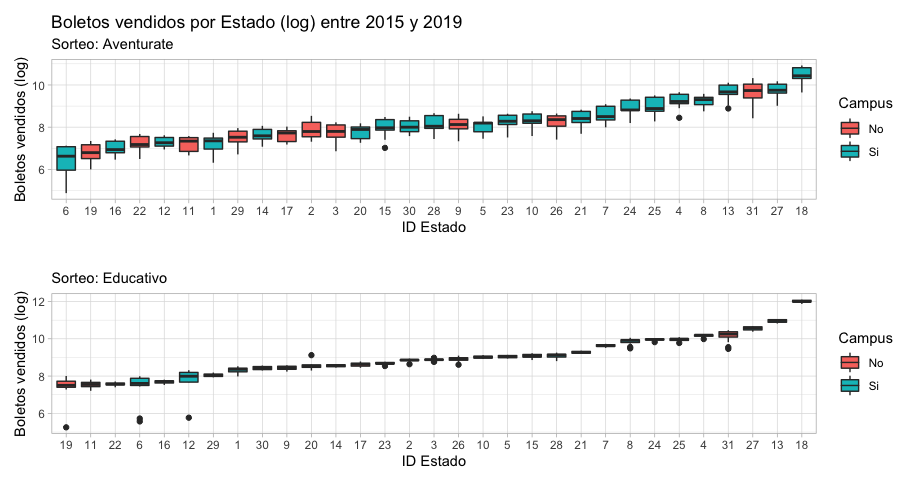
\includegraphics[scale = 0.43]{Imagenes/boxplot1.png}
    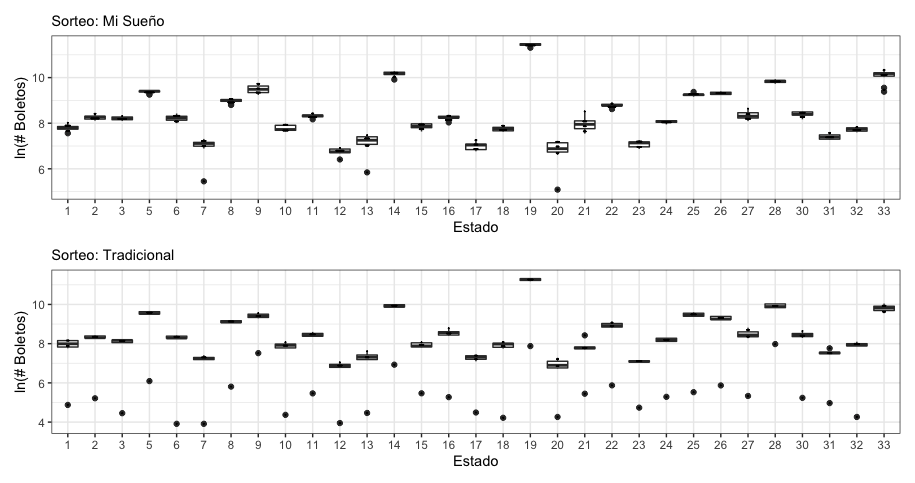
\includegraphics[scale = 0.43]{Imagenes/boxplot2.png}
    \centering
    \imagesource{Elaboración propia}
\end{figure}

\newpage

Inicialmente, se buscó encontrar la relación existente entre el número de boletos vendidos y el PIB \textit{per capita} para cada sorteo. Se aplicó logarítmos a ambos ejes.

\begin{figure}[H]
    \caption{Boletos vs PIB \textit{per capita}}
    \label{fig:scat}
    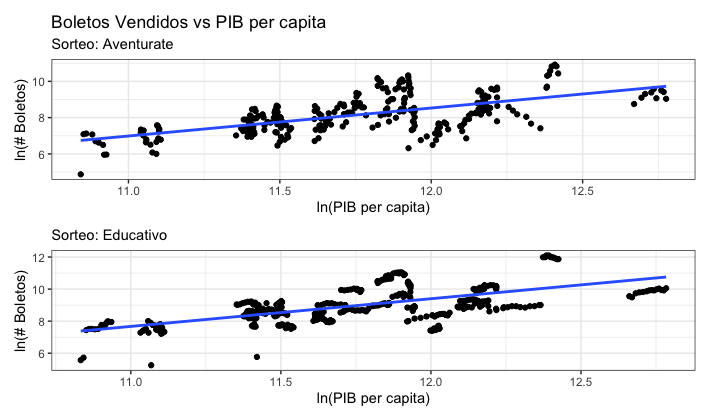
\includegraphics[scale = 0.35]{Imagenes/yvsx1.png}
    \centering
    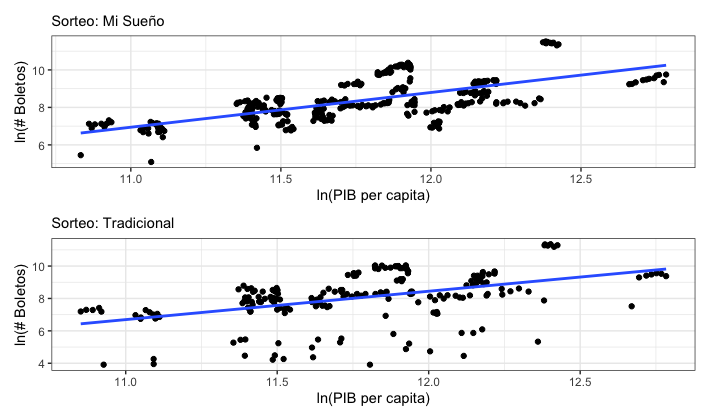
\includegraphics[scale = 0.35]{Imagenes/yvsx2.png} \\
    \centering
    \imagesource{Elaboración propia}
\end{figure}

De las gráficas anteriores, se observa una clara relación positiva entre el logaritmo natural del número de boletos vendidos y el logaritmo natural del PIB \textit{per capita}. Esto resulta relevante pues, como se mencionó en el capítulo anterior, la elasticidad ingreso nos mide la sensibilidad en la cantidad demandada de un bien cuando cambia el ingreso. Observar esta relación positiva nos empieza a dar señales de cómo será esta elasticidad. \\

Por otro lado, observamos que para los cuatro sorteos el Estado en donde se registraron el mayor número de boletos vendidos fue Nuevo León. Un aspecto relevante es que entre los años 2015 y 2019 Nuevo León fue el tercer Estado con un PIB promedio más alto como se ve en la siguiente gráfica.

\begin{figure}[H]
    \centering
    \caption{PIB por Estado}
    \label{fig:box-pib}
    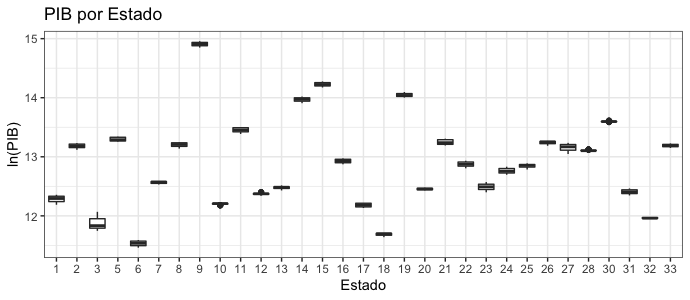
\includegraphics[scale = 0.5]{Imagenes/boxplot_pib.png}
    \imagesource{Elaboración propia}
\end{figure}

%Escribir sobre los datos, que estado tiene el maximo en boletos vendidos y el que tiene mayor pib etc!!!!




\newpage

\section{Modelo}

\noindent Para la comprobación de la hipótesis propuesta para esta tesis, se corrieron diferentes modelos de regresión tanto lineal simple como múltiple. \\

Los modelos econométricos que se utilizarán en este trabajo son los siguientes:

\begin{equation}
    ln(y) = \beta_0 + \beta_1 ln(x) + \epsilon
\end{equation}

\begin{equation}
    y = \beta_0 + \beta_1 x + \beta_2 x^2 + \epsilon
\end{equation}
 
Donde $y$ es el número de boletos vendidos, $x$ es el PIB \textit{per capita} y $\epsilon \sim N(0,1)$ para ambos modelos. Estos modelos nos servirán para encontrar con la ecuación (3.1) la elasticidad ingreso y con la ecuación (3.2) la concavidad de la función. \\

En un modelo de la forma $y = \beta_0 + \beta_1 x + \varepsilon$ el coeficiente $\beta_1 = \frac{\partial y}{\partial x}$, si tomamos el modelo (3.1) el coeficiente $\beta_1$ toma mayor relevancia pues $\beta_1 = \frac{\partial \% y}{\partial \% x}$. Traduciendolo a nuestro contexto con nuestras variables tenemos que,

\begin{equation*}
    \beta_1 = \frac{\Delta \% boletos}{\Delta \% PIB pc} \equiv \varepsilon_{I,x}
\end{equation*} \\

Así, obtenemos la elasticidad ingreso de los boletos del Sorteo Tec la cual es parte central de nuestra investigación. Ahora, el modelo (3.2) nos explicará si existe una forma funcional cóncava o convexa, esto se obtiene del coeficiente $\beta_2 = \frac{\partial^2 y}{\partial x^2}$ del cual nos interesa el signo. Traduciéndolo a nuestro contexto con nuestras variables, tenemos que:

\begin{equation*}
    \beta_2 = \frac{\partial^2 boletos}{\partial PIBpc^2}
\end{equation*}

Si $\beta_2 < 0$ tenemos una función cóncava y si $\beta_2 > 0$ tenemos una función convexa. Bajo nuestra hipótesis, esperaríamos que la función fuera cóncava lo cual nos daría una idea de que el individuo es averso al riesgo como se explicó en el capítulo \textbf{2.1}. \\

Estos modelos se utilizarán para los cuatro sorteos y así analizar cada uno por separado. A continuación, en el cuadro 3.2 se presenta el ajuste que se realizó para el modelo (3.1) y en el cuadro 3.3 se presenta el ajuste que se realizó para el modelo (3.2). La validación de los modelos se encuentra en el apéndice A. \\

%Regresiones para los 4 sorteos: modelo ln(y) ~ ln(x)
\begin{table}[H] 
\centering 
  \caption{Ajuste modelo (3.1)} 
  \label{lm-log} 
\begin{tabular}{@{\extracolsep{5pt}}lcc} 
\\[-1.8ex]\hline 
\hline \\[-1.8ex] 
 & \multicolumn{2}{c}{\textit{Dependent variable:}} \\ 
\cline{2-3} 
\\[-1.8ex] & \multicolumn{2}{c}{ln(\# Boletos)} \\ 
\\[-1.8ex] & AventuraT & Educativo\\ 
\hline \\[-1.8ex] 
 ln(PIB pc) & 1.542$^{***}$ &  \\ 
  & (0.120) &  \\ 
  & & \\ 
 ln(PIB pc) &  & 1.726$^{***}$ \\ 
  &  & (0.103) \\ 
  & & \\ 
 Constant & $-$9.979$^{***}$ & $-$11.317$^{***}$ \\ 
  & (1.417) & (1.211) \\ 
  & & \\ 
\hline \\[-1.8ex] 
R$^{2}$ & 0.372 & 0.395 \\ 
Adjusted R$^{2}$ & 0.370 & 0.393 \\ 
Residual Std. Error & 0.809 (df = 277) & 0.861 (df = 431) \\ 
F Statistic & 163.937$^{***}$ (df = 1; 277) & 281.194$^{***}$ (df = 1; 431) \\ 
\hline 
\hline \\[-1.8ex] 
\textit{Note:}  & \multicolumn{2}{r}{$^{*}$p$<$0.1; $^{**}$p$<$0.05; $^{***}$p$<$0.01} \\ 
\end{tabular} 
\end{table}

\begin{table}[H]
\centering 
  %\caption{} 
  %\label{} 
\begin{tabular}{@{\extracolsep{5pt}}lcc} 
\\[-1.8ex]\hline 
\hline \\[-1.8ex] 
 & \multicolumn{2}{c}{\textit{Dependent variable:}} \\ 
\cline{2-3} 
\\[-1.8ex] & \multicolumn{2}{c}{ln(\# Boletos)} \\ 
\\[-1.8ex] & Mi Sueño & Tradicional\\ 
\hline \\[-1.8ex] 
 ln(PIB pc) & 1.854$^{***}$ &  \\ 
  & (0.113) &  \\ 
  & & \\ 
 ln(PIB pc) &  & 1.751$^{***}$ \\ 
  &  & (0.232) \\ 
  & & \\ 
 Constant & $-$13.448$^{***}$ & $-$12.565$^{***}$ \\ 
  & (1.335) & (2.728) \\ 
  & & \\ 
\hline \\[-1.8ex] 
R$^{2}$ & 0.441 & 0.212 \\ 
Adjusted R$^{2}$ & 0.440 & 0.209 \\ 
Residual Std. Error & 0.835 (df = 338) & 1.345 (df = 212) \\ 
F Statistic & 266.968$^{***}$ (df = 1; 338) & 57.111$^{***}$ (df = 1; 212) \\ 
\hline 
\hline \\[-1.8ex] 
\textit{Note:}  & \multicolumn{2}{r}{$^{*}$p$<$0.1; $^{**}$p$<$0.05; $^{***}$p$<$0.01} \\ 
\end{tabular} 
\end{table}

%Regresiones para los 4 sorteos: modelo y ~ x + x^2

\begin{table}[H]
\centering 
  \caption{Ajuste modelo (3.2)} 
  \label{lm-x2} 
\begin{tabular}{@{\extracolsep{5pt}}lcc} 
\\[-1.8ex]\hline 
\hline \\[-1.8ex] 
 & \multicolumn{2}{c}{\textit{Dependent variable:}} \\ 
\cline{2-3} 
\\[-1.8ex] & \multicolumn{2}{c}{\# Boletos} \\ 
\\[-1.8ex] & AventuraT & Educativo\\ 
\hline \\[-1.8ex] 
 PIB pc & 0.120$^{***}$ &  \\ 
  & (0.028) &  \\ 
  & & \\ 
 PIB pc^2 & $-$1.613e-07$^{**}$ &  \\ 
  & (7.606e-08) &  \\ 
  & & \\ 
 PIB pc &  & 0.418$^{***}$ \\ 
  &  & (0.084) \\ 
  & & \\ 
 PIB pc^2 &  & $-$5.713e-07$^{**}$ \\ 
  &  & (2.291e-07) \\ 
  & & \\ 
 Constant & $-$6,909.530$^{***}$ & $-$28,626.400$^{***}$ \\ 
  & (2,285.693) & (6,858.514) \\ 
  & & \\ 
\hline \\[-1.8ex] 
R$^{2}$ & 0.222 & 0.194 \\ 
Adjusted R$^{2}$ & 0.216 & 0.191 \\ 
Residual Std. Error & 7,136.310 (df = 276) & 26,589.100 (df = 430) \\ 
F Statistic & 39.377$^{***}$ (df = 2; 276) & 51.861$^{***}$ (df = 2; 430) \\ 
\hline 
\hline \\[-1.8ex] 
\textit{Note:}  & \multicolumn{2}{r}{$^{*}$p$<$0.1; $^{**}$p$<$0.05; $^{***}$p$<$0.01} \\ 
\end{tabular} 
\end{table}

\begin{table}[H]
\centering 
%  \caption{} 
%  \label{} 
\begin{tabular}{@{\extracolsep{5pt}}lcc} 
\\[-1.8ex]\hline 
\hline \\[-1.8ex] 
 & \multicolumn{2}{c}{\textit{Dependent variable:}} \\ 
\cline{2-3} 
\\[-1.8ex] & \multicolumn{2}{c}{\# Boletos} \\ 
\\[-1.8ex] & Mi Sueño & Tradicional\\ 
\hline \\[-1.8ex] 
 PIB pc & 0.221$^{***}$ &  \\ 
  & (0.054) &  \\ 
  & & \\ 
 PIB pc^2 & $-$2.588e-07$^{*}$ &  \\ 
  & (1.471e-07) &  \\ 
  & & \\ 
 PIB pc &  & 0.180$^{***}$ \\ 
  &  & (0.055) \\ 
  & & \\ 
 PIB pc^2 &  & $-$2.253e-07 \\ 
  &  & (1.500e-07) \\ 
  & & \\ 
 Constant & $-$15,784.160$^{***}$ & $-$12,206.960$^{***}$ \\ 
  & (4,410.503) & (4,575.598) \\ 
  & & \\ 
\hline \\[-1.8ex] 
R$^{2}$ & 0.208 & 0.191 \\ 
Adjusted R$^{2}$ & 0.204 & 0.184 \\ 
Residual Std. Error & 15,011.720 (df = 337) & 12,282.270 (df = 211) \\ 
F Statistic & 44.358$^{***}$ (df = 2; 337) & 24.948$^{***}$ (df = 2; 211) \\ 
\hline 
\hline \\[-1.8ex] 
\textit{Note:}  & \multicolumn{2}{r}{$^{*}$p$<$0.1; $^{**}$p$<$0.05; $^{***}$p$<$0.01} \\ 
\end{tabular} 
\end{table}




% Para escribir ecuaciones

%\begin{table}[H]
%\centering
%\caption{Resultados del modelo econométrico}
%\label{REG}
%\begin{tabular}{|ccccc|}
%  \hline
% & Estimador & Desv. est. & Valor $t$ & Pr($>|t|$) \\ 
%  \hline
%  $\alpha$ & x & x & x & x \\ 
%  CI & x & x & x & x \\ 
%  IS & x & x & x & x \\ 
%  IR & x & x & x & x \\ 
%  PT & x & x & x & x \\ 
%   \hline
%\multicolumn{5}{|c|}{Error est. de res. = x con x gr. de libertad}
%    \\
%    \multicolumn{5}{|c|}{$R^2$ = x y $\bar{R}^2$ = x}
% \\
% \multicolumn{5}{|c|}{Estadístico $F$ = x, con un valor $p$ = x }
%      \\
%\hline
%\end{tabular} \\

%\end{table}
